\documentclass[aspectratio=169,11pt]{beamer}

\usepackage{fontspec}
\IfFontExistsTF{Arial}{\setsansfont{Arial}}{\setsansfont{TeX Gyre Heros}}
\usepackage{amsmath,amssymb}
\usepackage{graphicx}
\usepackage{booktabs,tabularx,array}
\usepackage{tikz}
\usetikzlibrary{arrows.meta,positioning,calc}
\usepackage{ragged2e}
\usepackage{adjustbox}
\usepackage{pgfpages}

\newif\ifshownotes
\ifdefined\EnableNotes\shownotestrue\else\shownotesfalse\fi
\ifshownotes
  \setbeameroption{show notes on second screen=right}
  \setbeamerfont{note page}{size={\fontsize{7}{8}\selectfont}}
\else
  \setbeameroption{hide notes}
\fi

\definecolor{UoGRed}{HTML}{CC0000}
\definecolor{UoGDarkGray}{HTML}{505050}
\definecolor{UoGTextGray}{HTML}{555555}
\definecolor{UoGLightGray}{HTML}{E9E9E9}
\definecolor{UoGBlue}{HTML}{2F75B5}

\setbeamercolor{normal text}{fg=black,bg=white}
\setbeamercolor{structure}{fg=UoGRed}
\setbeamercolor{frametitle}{fg=black,bg=white}
\setbeamercolor{alerted text}{fg=UoGRed}
\setbeamerfont{frametitle}{series=\bfseries,size={\fontsize{17}{19}\selectfont}}
\setbeamerfont{normal text}{size=\normalsize}
\setbeamertemplate{navigation symbols}{}
\setbeamersize{text margin left=0.58cm,text margin right=0.58cm}

\setbeamertemplate{headline}{%
  \begin{beamercolorbox}[wd=\paperwidth,ht=1.03cm,dp=0cm]{normal text}
    \hspace*{0.46cm}\raisebox{0.13cm}{
\includegraphics[height=0.70cm]{assets/uog-logo.png}}
  \end{beamercolorbox}%
  \begin{beamercolorbox}[wd=\paperwidth,ht=0.20cm,dp=0cm]{structure}
    \color{UoGRed}\rule{\paperwidth}{0.20cm}%
    \hspace*{-1.40cm}\raisebox{0.03cm}{\color{white}\scriptsize\insertframenumber}
  \end{beamercolorbox}%
}

\setbeamertemplate{frametitle}{%
  \vspace*{0.05cm}%
  \nointerlineskip
  \begin{beamercolorbox}[wd=\textwidth,sep=0.04cm,dp=0.05cm,left]{frametitle}
    \usebeamerfont{frametitle}\insertframetitle
  \end{beamercolorbox}%
}

\setbeamertemplate{footline}{}

\newcommand{\UoGTakeaway}[1]{%
  \begin{beamercolorbox}[wd=\linewidth,sep=0.16cm,center]{normal text}
    \colorbox{UoGDarkGray}{\parbox{0.965\linewidth}{\centering\color{white}\bfseries #1}}
  \end{beamercolorbox}%
}

\newcommand{\TalkSource}[1]{%
  \vfill\hfill{\fontsize{5.5}{6.2}\selectfont\color{UoGTextGray}Source: #1}%
}

\newif\ifdraftmode
\draftmodefalse
\newcommand{\TalkTODO}[1]{%
  \ifdraftmode
    \par\smallskip\colorbox{yellow!35}{\parbox{0.95\linewidth}{\scriptsize\textbf{TODO:} #1}}%
  \fi
}

\newcommand{\RedLabel}[1]{\textcolor{UoGRed}{\bfseries #1}}
\newcommand{\MethodArrow}{\tikz[baseline=-0.5ex]\draw[->,line width=0.8pt,UoGRed] (0,0)--(0.55,0);}

\graphicspath{{../}{assets/}}

\title{Control of Mixed-Autonomy Traffic via Autonomous Vehicles with Lane-Changing Behavior}
\author{Shuwei Pei \and Muhammed O. Sayin \and Saeed Ahmed}
\institute{University of Groningen \textperiodcentered{} Bilkent University}
\date{23rd IFAC World Congress \textperiodcentered{} Busan \textperiodcentered{} 23--28 August 2026}

\begin{document}

% -----------------------------------------------------------------------------
% Slide 1
% -----------------------------------------------------------------------------
\begin{frame}[plain]
  \begin{tikzpicture}[remember picture,overlay]
    \node[anchor=north west,inner sep=0] at ([xshift=0.45cm,yshift=-0.22cm]current page.north west)
      {
\includegraphics[height=0.72cm]{assets/uog-logo.png}};
    \fill[UoGRed] ([yshift=-1.08cm]current page.north west) rectangle ([yshift=-1.28cm]current page.north east);
    \fill[UoGDarkGray] ([yshift=-1.45cm]current page.north west) rectangle ([yshift=-4.06cm]current page.north east);
    \node[anchor=west,text width=14.9cm,align=left] at ([xshift=0.72cm,yshift=-2.76cm]current page.north west) {
      \fontsize{18}{21}\selectfont\bfseries\color{white}
      Control of Mixed-Autonomy Traffic via\\
      Autonomous Vehicles with Lane-Changing\\
      Behavior
    };
    \node[anchor=west,text width=14.5cm,align=left] at ([xshift=0.72cm,yshift=1.78cm]current page.south west) {
      \large\bfseries Shuwei Pei, Muhammed O. Sayin, and Saeed Ahmed\\[0.14cm]
      \normalsize University of Groningen \textperiodcentered{} Bilkent University\\[0.14cm]
      \normalsize 23rd IFAC World Congress \textperiodcentered{} Busan \textperiodcentered{} 23--28 August 2026
    };
  \end{tikzpicture}
  \note{
    \textbf{Timing:} 0:30

    \textbf{Opening.} Good morning. I am Shuwei Pei from the University of Groningen. This is joint work with Muhammed O. Sayin from Bilkent University and Saeed Ahmed from the University of Groningen.

    \textbf{Main explanation.} We study how human lane-changing changes the classical traffic-stabilization problem. The focus of this talk is the methodological derivation: from problem formulation, through reinforcement learning, to an interpretable rule-based controller.

    \textbf{Scientific interpretation.} The final controller is not introduced as an isolated heuristic. It is derived from a sequence of controlled learning experiments.

    \textbf{Transition.} I will begin with why lane-changing changes the nature of the control problem.

    \textbf{Likely question.} Is the final controller learned? No. RL is used as a design instrument; the deployed PARC controller is rule-based.

    \textbf{Sources.} Docs/ifacconf8pages.tex, title and author block; official IFAC 2026 congress information; UoG-Wide.pptx.
  }
\end{frame}

% -----------------------------------------------------------------------------
% Slide 2
% -----------------------------------------------------------------------------
\begin{frame}[shrink=8]{Stop-and-go waves become a two-dimensional control problem}
  \begin{columns}[T,onlytextwidth]
    \begin{column}{0.39\textwidth}
      \footnotesize
      \textbf{Stop-and-go waves are usually treated as a longitudinal-control problem.}

      \smallskip
      \textcolor{UoGRed}{\bfseries Human lane-changing adds a second disturbance channel.}

      \smallskip
      \begin{itemize}\setlength\itemsep{0.07cm}
        \item Small braking disturbances propagate upstream.
        \item Lane changes abruptly modify leader--follower relationships.
        \item A controller confined to one lane cannot reject disturbances entering from another lane.
      \end{itemize}
    \end{column}
    \begin{column}{0.59\textwidth}
      \centering
      \begin{tikzpicture}
        \node[inner sep=0] (wave) {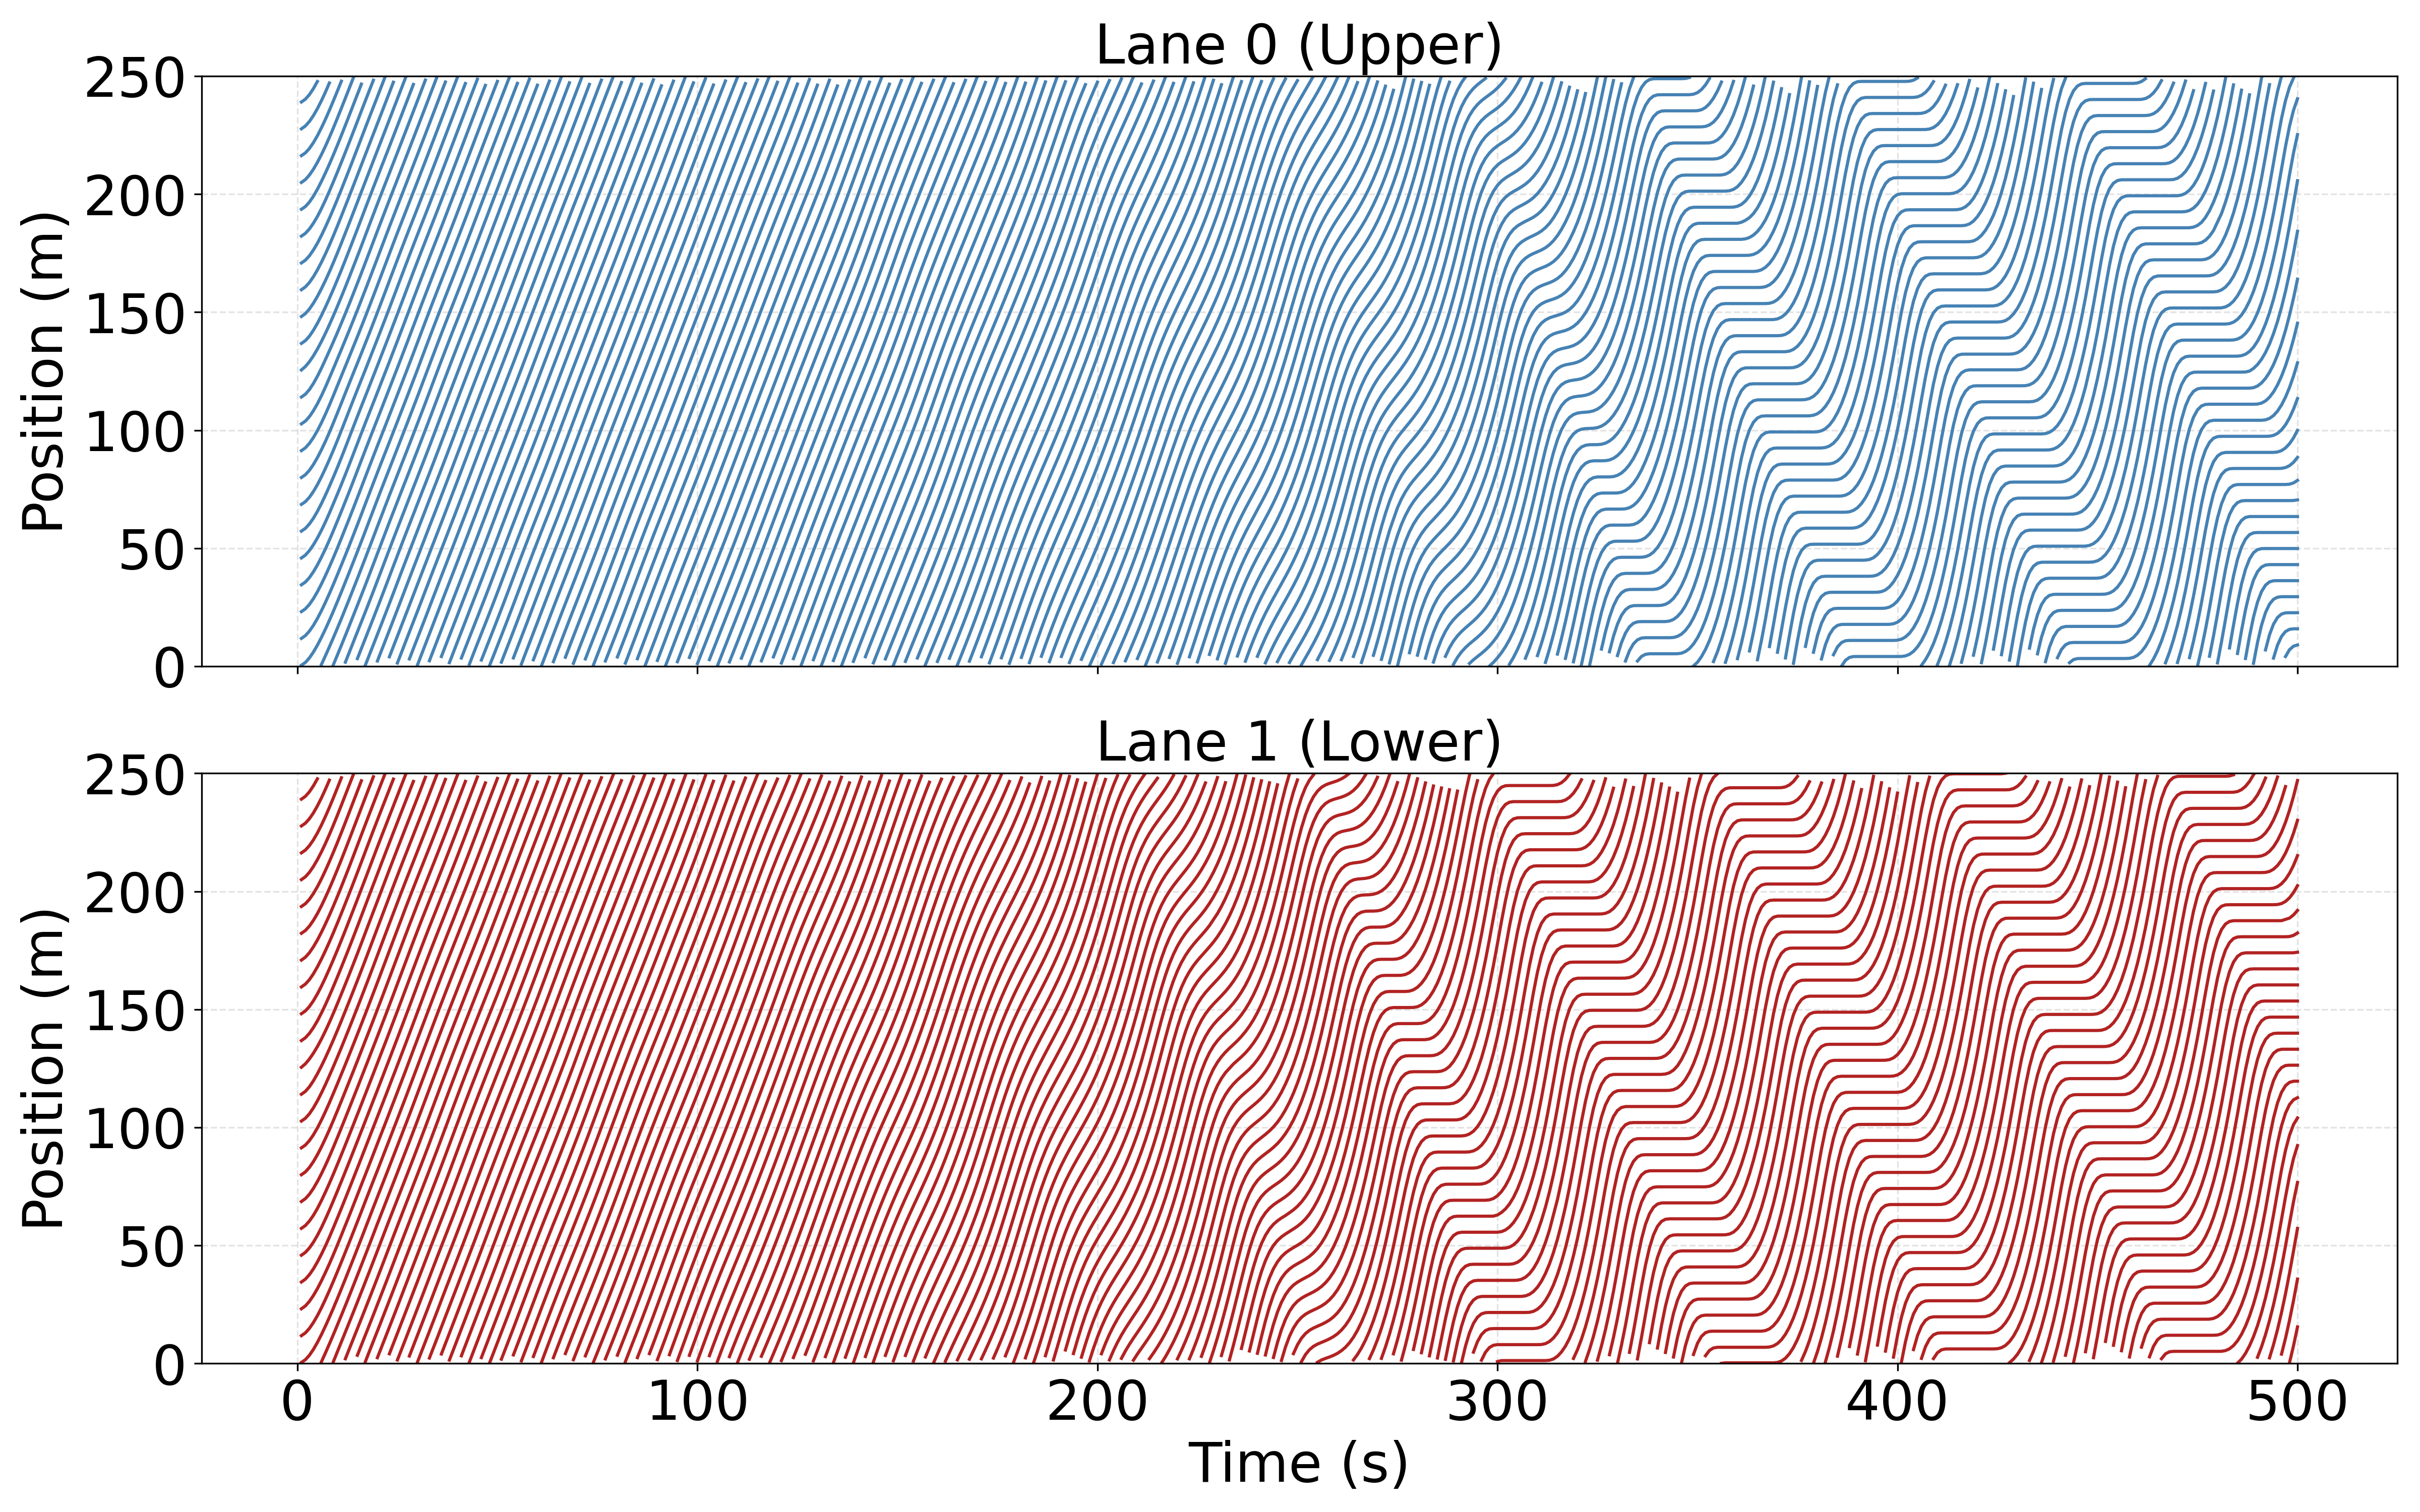
\includegraphics[width=\linewidth,height=3.65cm,keepaspectratio]{../trajectory_log_allhuman44.png}};
        \draw[overlay,-{Latex[length=2mm]},UoGRed,line width=0.8pt] ($(wave.north west)+(3.8,-1.15)$) -- ++(-0.65,-0.42);
        \node[overlay,fill=white,draw=UoGRed,rounded corners=1pt,font=\scriptsize,anchor=west] at ($(wave.north west)+(3.75,-1.10)$) {Stop-and-go wave};
      \end{tikzpicture}
      \par\smallskip
      \scriptsize\color{UoGTextGray}Lane-changing changes the active leader--follower graph.
    \end{column}
  \end{columns}
  \vspace{0.05cm}
  \UoGTakeaway{Local longitudinal stabilization does not guarantee multi-lane system stability.}
  \TalkSource{Paper: Introduction and Problem Formulation; trajectory\_log\_allhuman44.png}
  \note{
    \textbf{Timing:} 0:50

    \textbf{Opening.} Stop-and-go oscillations are repeated vehicle deceleration and acceleration rather than steady motion.

    \textbf{Main explanation.} A braking disturbance propagates upstream through car-following interactions. A lane change does more than move one vehicle laterally: it changes which vehicles interact longitudinally. This creates a hybrid, cross-lane disturbance channel.

    \textbf{Scientific interpretation.} A controller may stabilize its own local platoon while the complete two-lane system remains unstable. Local longitudinal stabilization is therefore not equivalent to multi-lane system stability.

    \textbf{Transition.} This limitation becomes clearer when we compare the main control paradigms used in traffic research.

    \textbf{Likely question.} Are all lane changes undesirable? No. The controlled ring isolates unnecessary, destabilizing lane changes in dense traffic; necessary route-following lane changes remain a separate problem.

    \textbf{Sources.} Docs/ifacconf8pages.tex, Introduction and Problem Formulation; Docs/trajectory\_log\_allhuman44.png.
  }
\end{frame}

% -----------------------------------------------------------------------------
% Slide 3
% -----------------------------------------------------------------------------
\begin{frame}[shrink=8]{Existing methods solve different parts of the problem}
  \small
  \renewcommand{\arraystretch}{1.55}
  \begin{tabularx}{\linewidth}{>{\bfseries\raggedright\arraybackslash}p{0.19\linewidth} >{\raggedright\arraybackslash}p{0.27\linewidth} >{\raggedright\arraybackslash}X}
    \toprule
    \textcolor{UoGRed}{Paradigm} & \textcolor{UoGRed}{Strength} & \textcolor{UoGRed}{Limitation for this problem}\\
    \midrule
    Rule-based control & Interpretable and deployable & Usually designed for longitudinal regulation within one lane\\
    Optimization-based control & Handles models and constraints explicitly & Requires repeated solution of a potentially expensive optimization problem\\
    Learning-based control & Can adapt to complex HDV interactions & Learned policies may be difficult to interpret and generalize\\
    \bottomrule
  \end{tabularx}
  \vspace{0.28cm}
  \UoGTakeaway{The missing element is an interpretable controller that explicitly coordinates traffic across lanes.}
  \TalkSource{Paper: Introduction and cited ACC/CACC, MPC, Flow, and RL literature}
  \note{
    \textbf{Timing:} 1:00

    \textbf{Opening.} The paper positions the problem across three established traffic-control paradigms.

    \textbf{Main explanation.} Rule-based methods such as ACC and CACC are attractive because they are interpretable and deployable. Optimization-based approaches, including MPC and robust control, can explicitly handle objectives and constraints but introduce computational and modeling requirements. Learning-based approaches can adapt to complex HDV interactions, although the resulting policies may be difficult to interpret.

    \textbf{Scientific interpretation.} We use RL as a scientific policy-search and mechanism-discovery tool. The missing element is an interpretable controller that coordinates traffic explicitly across lanes.

    \textbf{Transition.} This leads to three methodological questions that organize the complete study.

    \textbf{Likely question.} Why not start directly with MPC? The purpose of this paper is to identify a useful coordination structure experimentally before constructing a transparent rule-based controller.

    \textbf{Sources.} Docs/ifacconf8pages.tex, Introduction and cited literature.
  }
\end{frame}

% -----------------------------------------------------------------------------
% Slide 4
% -----------------------------------------------------------------------------
\begin{frame}{The study follows three methodological questions}
  \begin{enumerate}\setlength\itemsep{0.45cm}
    \item[\RedLabel{Q1.}] \textbf{Can one RL-controlled AV stabilize two-lane traffic when HDVs change lanes?}
    \item[\RedLabel{Q2.}] \textbf{What coordination structure appears when two AVs share information?}
    \item[\RedLabel{Q3.}] \textbf{Can that structure be converted into an interpretable rule-based controller?}
  \end{enumerate}

  \vspace{0.42cm}
  \centering
  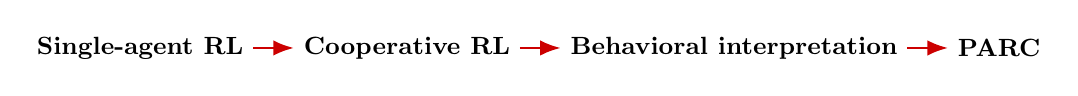
\begin{tikzpicture}[node distance=0.52cm, every node/.style={font=\small\bfseries,align=center}]
    \node (a) {Single-agent RL};
    \node[right=of a] (b) {Cooperative RL};
    \node[right=of b] (c) {Behavioral interpretation};
    \node[right=of c] (d) {PARC};
    \draw[-{Latex},UoGRed,line width=1.0pt] (a)--(b);
    \draw[-{Latex},UoGRed,line width=1.0pt] (b)--(c);
    \draw[-{Latex},UoGRed,line width=1.0pt] (c)--(d);
  \end{tikzpicture}
  \TalkSource{Paper: contribution and organization paragraphs}
  \note{
    \textbf{Timing:} 0:45

    \textbf{Opening.} The paper does not begin by assuming PARC is the correct controller.

    \textbf{Main explanation.} The first experiment tests whether the classical single-AV result generalizes to lane-changing traffic. The second changes the information and control architecture by introducing two coordinated AVs. The third interprets the learned behavior and converts it into a transparent controller.

    \textbf{Scientific interpretation.} The sequence separates failure diagnosis, behavior discovery, and controller design. The final controller does not require RL inference at runtime.

    \textbf{Transition.} To answer these questions, we first construct a controlled two-lane testbed.

    \textbf{Likely question.} Was pairing specified from the beginning? Pairing is encouraged by the cooperative reward, but the rule-based controller is constructed only after interpreting the trained policy behavior.

    \textbf{Sources.} Docs/ifacconf8pages.tex, contribution and organization paragraphs.
  }
\end{frame}

% -----------------------------------------------------------------------------
% Slide 5
% -----------------------------------------------------------------------------
\begin{frame}[shrink=8]{A controlled testbed isolates lane-changing disturbances}
  \begin{columns}[T,onlytextwidth]
    \begin{column}{0.47\textwidth}
      \centering
      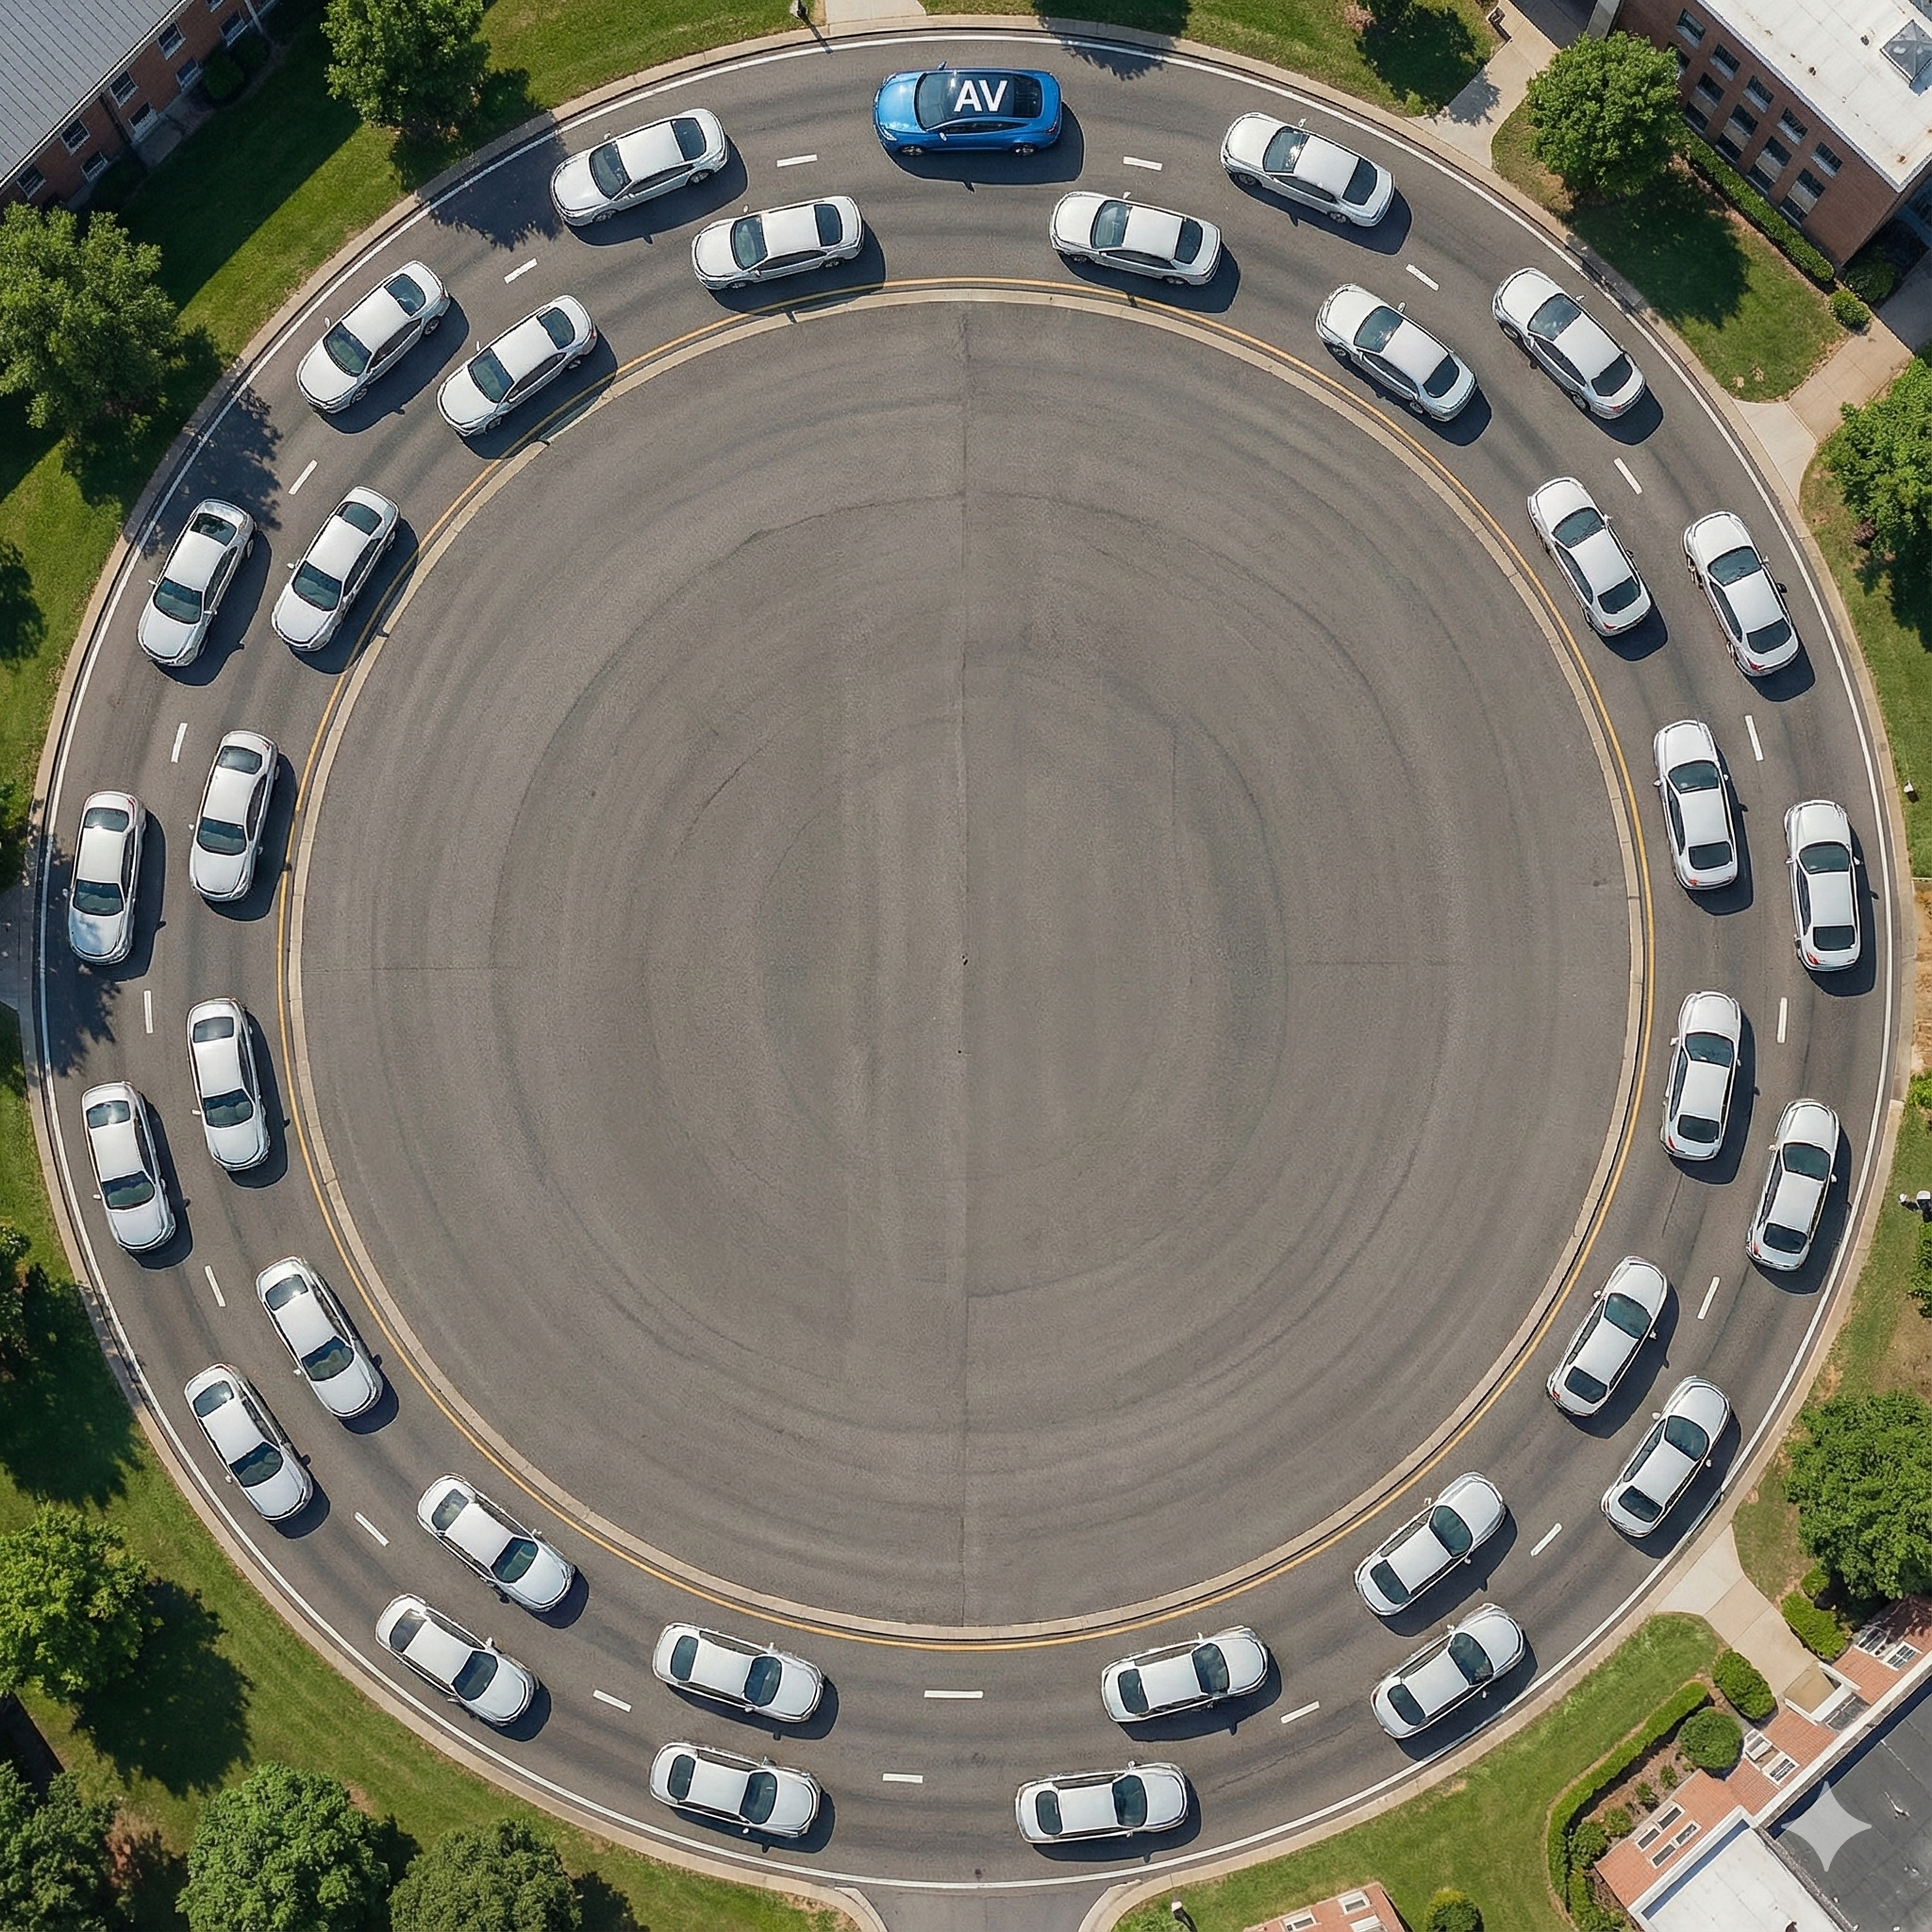
\includegraphics[width=0.88\linewidth,height=4.55cm,keepaspectratio]{../doublelaneringnetwork_2.png}
    \end{column}
    \begin{column}{0.51\textwidth}
      \footnotesize
      \begin{itemize}\setlength\itemsep{0.08cm}
        \item Two-lane ring road, $L=250\,\mathrm{m}$
        \item $N_{\mathrm{total}}=44$ vehicles
        \item SUMO microscopic simulation
        \item Flow reinforcement-learning interface
        \item IDM longitudinal dynamics
        \item Heterogeneous LC2013 lane-changing behavior
        \item Bounded AV acceleration commands
      \end{itemize}
      \vspace{0.10cm}
      \begin{tabularx}{\linewidth}{@{}p{0.16\linewidth}X@{}}
        \RedLabel{HDVs:} & IDM + LC2013\\
        \RedLabel{AVs:} & learned or rule-based longitudinal control
      \end{tabularx}
    \end{column}
  \end{columns}
  \UoGTakeaway{The ring removes boundary-flow effects and isolates cross-lane interactions.}
  \TalkTODO{Unify the warm-up convention before a final experimental revision.}
  \TalkSource{Paper: Simulation Setup; Flow/SUMO configurations; doublelaneringnetwork\_2.png}
  \note{
    \textbf{Timing:} 1:00

    \textbf{Opening.} The ring maintains a controlled traffic density and removes inflow and outflow boundary effects.

    \textbf{Main explanation.} The network has two 250-metre lanes and 44 vehicles in total. SUMO supplies microscopic traffic dynamics and Flow connects the RL policy. HDVs use longitudinal car-following behavior and LC2013 lane-changing. Randomized driver parameters create heterogeneous behavior.

    \textbf{Scientific interpretation.} Oscillations are established before active controller performance is evaluated. I avoid stating one common warm-up duration because the rule-based configurations use 5000 steps at 0.1 seconds while some RL configurations use 2000 steps at 0.1 seconds.

    \textbf{Transition.} We represent the resulting sequential decision problem as a Markov decision process.

    \textbf{Likely question.} Are there exactly 22 vehicles in each lane? The study uses 44 vehicles on two lanes, but the configurations do not support that wording uniformly across every run.

    \textbf{Sources.} Docs/ifacconf8pages.tex, Simulation Setup; paired\_ring.py; singleagent\_ring.py; singleagent\_ring2AV.py; Docs/doublelaneringnetwork\_2.png.
  }
\end{frame}

% -----------------------------------------------------------------------------
% Slide 6
% -----------------------------------------------------------------------------
\begin{frame}{We formulate traffic control as a finite-horizon MDP}
  \begin{columns}[T,onlytextwidth]
    \begin{column}{0.54\textwidth}
      \vspace{0.30cm}
      \begin{align*}
        \mathcal{M}&=(\mathcal{S},\mathcal{A},\mathcal{T},r,\rho_0,\gamma,H),\\[0.55cm]
        \max_{\pi}J(\pi)
        &=\mathbb{E}_{\pi,\mathcal{T}}
        \left[
          \sum_{t=0}^{H-1}\gamma^t r(s_t,a_t,s_{t+1})
        \right].
      \end{align*}
    \end{column}
    \begin{column}{0.44\textwidth}
      \begin{itemize}\setlength\itemsep{0.28cm}
        \item[\RedLabel{$\mathcal{S}$}] local traffic and AV coordination states
        \item[\RedLabel{$\mathcal{A}$}] AV acceleration and, where applicable, lane-change decisions
        \item[\RedLabel{$\mathcal{T}$}] stochastic SUMO traffic evolution
        \item[\RedLabel{$r$}] traffic efficiency and coordination objective
      \end{itemize}
    \end{column}
  \end{columns}
  \vspace{0.38cm}
  \UoGTakeaway{Observation, action, and reward design determine what coordination can be learned.}
  \TalkSource{Paper: Formulation as an RL Problem}
  \note{
    \textbf{Timing:} 0:50

    \textbf{Opening.} I will not give a general reinforcement-learning tutorial; I will map the MDP directly to this traffic problem.

    \textbf{Main explanation.} The state contains local traffic variables and, later, AV coordination variables. The action controls AV acceleration and, in the single-agent formulation, a lane-change decision. SUMO determines the stochastic state transition. The reward specifies traffic efficiency and coordination objectives.

    \textbf{Scientific interpretation.} The important design choices are observation, action, and reward. These choices determine both the information available to the policy and the coordination structures it can learn.

    \textbf{Transition.} The first formulation gives one AV information about both lanes but only one local actuator.

    \textbf{Likely question.} Is the problem actually infinite horizon? Conceptually yes; the implementation approximates it with a large finite horizon.

    \textbf{Sources.} Docs/ifacconf8pages.tex, Formulation as an RL Problem.
  }
\end{frame}

% -----------------------------------------------------------------------------
% Slide 7
% -----------------------------------------------------------------------------
\begin{frame}{The single AV observes both lanes but acts locally}
  \begin{columns}[T,onlytextwidth]
    \begin{column}{0.61\textwidth}
      \small
      \begin{align*}
        o_t&=\left[\frac{v_t^{\mathrm{AV}}}{v_{\max}},\mathbf z_t^{(0)},\mathbf z_t^{(1)}\right]\in\mathbb{R}^{11},\\[0.15cm]
        \mathbf z_t^{(\ell)}&=\left[
          \mathbf{1}_{\{\ell=\ell_t\}},
          \frac{d_{f,t}^{\ell}}{L},
          \frac{v_{f,t}^{\ell}}{v_{\max}},
          \frac{d_{b,t}^{\ell}}{L},
          \frac{v_{b,t}^{\ell}}{v_{\max}}
        \right],\\[0.15cm]
        a_t&=\left[a_t^{\mathrm{acc}},a_t^{\mathrm{lc,raw}}\right],\\[0.15cm]
        r_t&=\text{instantaneous average traffic speed}.
      \end{align*}
    \end{column}
    \begin{column}{0.37\textwidth}
      \centering
      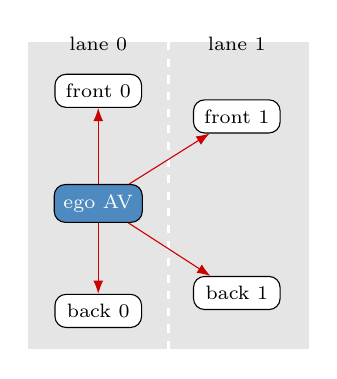
\begin{tikzpicture}[x=0.83cm,y=0.65cm,font=\scriptsize]
        \fill[black!10] (0,0) rectangle (4.3,6.0);
        \draw[white,line width=1.2pt,dashed] (2.15,0)--(2.15,6.0);
        \node[draw,rounded corners,fill=UoGBlue!85,text=white,minimum width=1.10cm,minimum height=0.48cm] (ego) at (1.08,2.85) {ego AV};
        \node[draw,rounded corners,fill=white,minimum width=1.10cm,minimum height=0.42cm] (f0) at (1.08,5.05) {front 0};
        \node[draw,rounded corners,fill=white,minimum width=1.10cm,minimum height=0.42cm] (b0) at (1.08,0.75) {back 0};
        \node[draw,rounded corners,fill=white,minimum width=1.10cm,minimum height=0.42cm] (f1) at (3.20,4.55) {front 1};
        \node[draw,rounded corners,fill=white,minimum width=1.10cm,minimum height=0.42cm] (b1) at (3.20,1.10) {back 1};
        \draw[-{Latex},UoGRed] (ego)--(f0);
        \draw[-{Latex},UoGRed] (ego)--(b0);
        \draw[-{Latex},UoGRed] (ego)--(f1);
        \draw[-{Latex},UoGRed] (ego)--(b1);
        \node[anchor=south] at (1.08,5.65) {lane 0};
        \node[anchor=south] at (3.20,5.65) {lane 1};
      \end{tikzpicture}
    \end{column}
  \end{columns}
  \UoGTakeaway{The reward is global, but the AV's physical authority remains local.}
  \TalkSource{Paper: Single-Agent Reinforcement Learning; singleagent\_ring.py}
  \note{
    \textbf{Timing:} 1:10

    \textbf{Opening.} The single AV observes both lanes but still acts as one local vehicle.

    \textbf{Main explanation.} The observation has dimension 11. The first element is normalized ego speed. Each lane contributes a lane indicator and normalized front and back distance and speed. The action contains continuous acceleration and a continuous lane-change intention that is mapped to a discrete lane command. The reward is the instantaneous average speed of all vehicles.

    \textbf{Scientific interpretation.} Although the reward is global, the AV's physical authority remains local. Richer information does not create a second actuator in the adjacent lane.

    \textbf{Transition.} Under these constraints, the learned policy adopts a rational local strategy.

    \textbf{Likely question.} Why include adjacent-lane observations? They allow the policy to anticipate nearby traffic and lane-change opportunities, but they cannot overcome the actuation limitation.

    \textbf{Sources.} Docs/ifacconf8pages.tex, Single-Agent Reinforcement Learning; examples/exp\_configs/rl/singleagent/singleagent\_ring.py.
  }
\end{frame}

% -----------------------------------------------------------------------------
% Slide 8
% -----------------------------------------------------------------------------
\begin{frame}[shrink=8]{The single-agent formulation produces a locally rational policy}
  \begin{columns}[T,onlytextwidth]
    \begin{column}{0.40\textwidth}
      \small
      \textbf{The AV learns to close the gap to its leader.}
      \vspace{0.28cm}
      \begin{enumerate}\setlength\itemsep{0.27cm}
        \item A larger gap attracts HDV lane changes.
        \item A merging HDV forces braking and reduces the AV reward.
        \item The AV protects its local gap---but cannot stabilize the adjacent lane.
      \end{enumerate}
    \end{column}
    \begin{column}{0.58\textwidth}
      \centering
      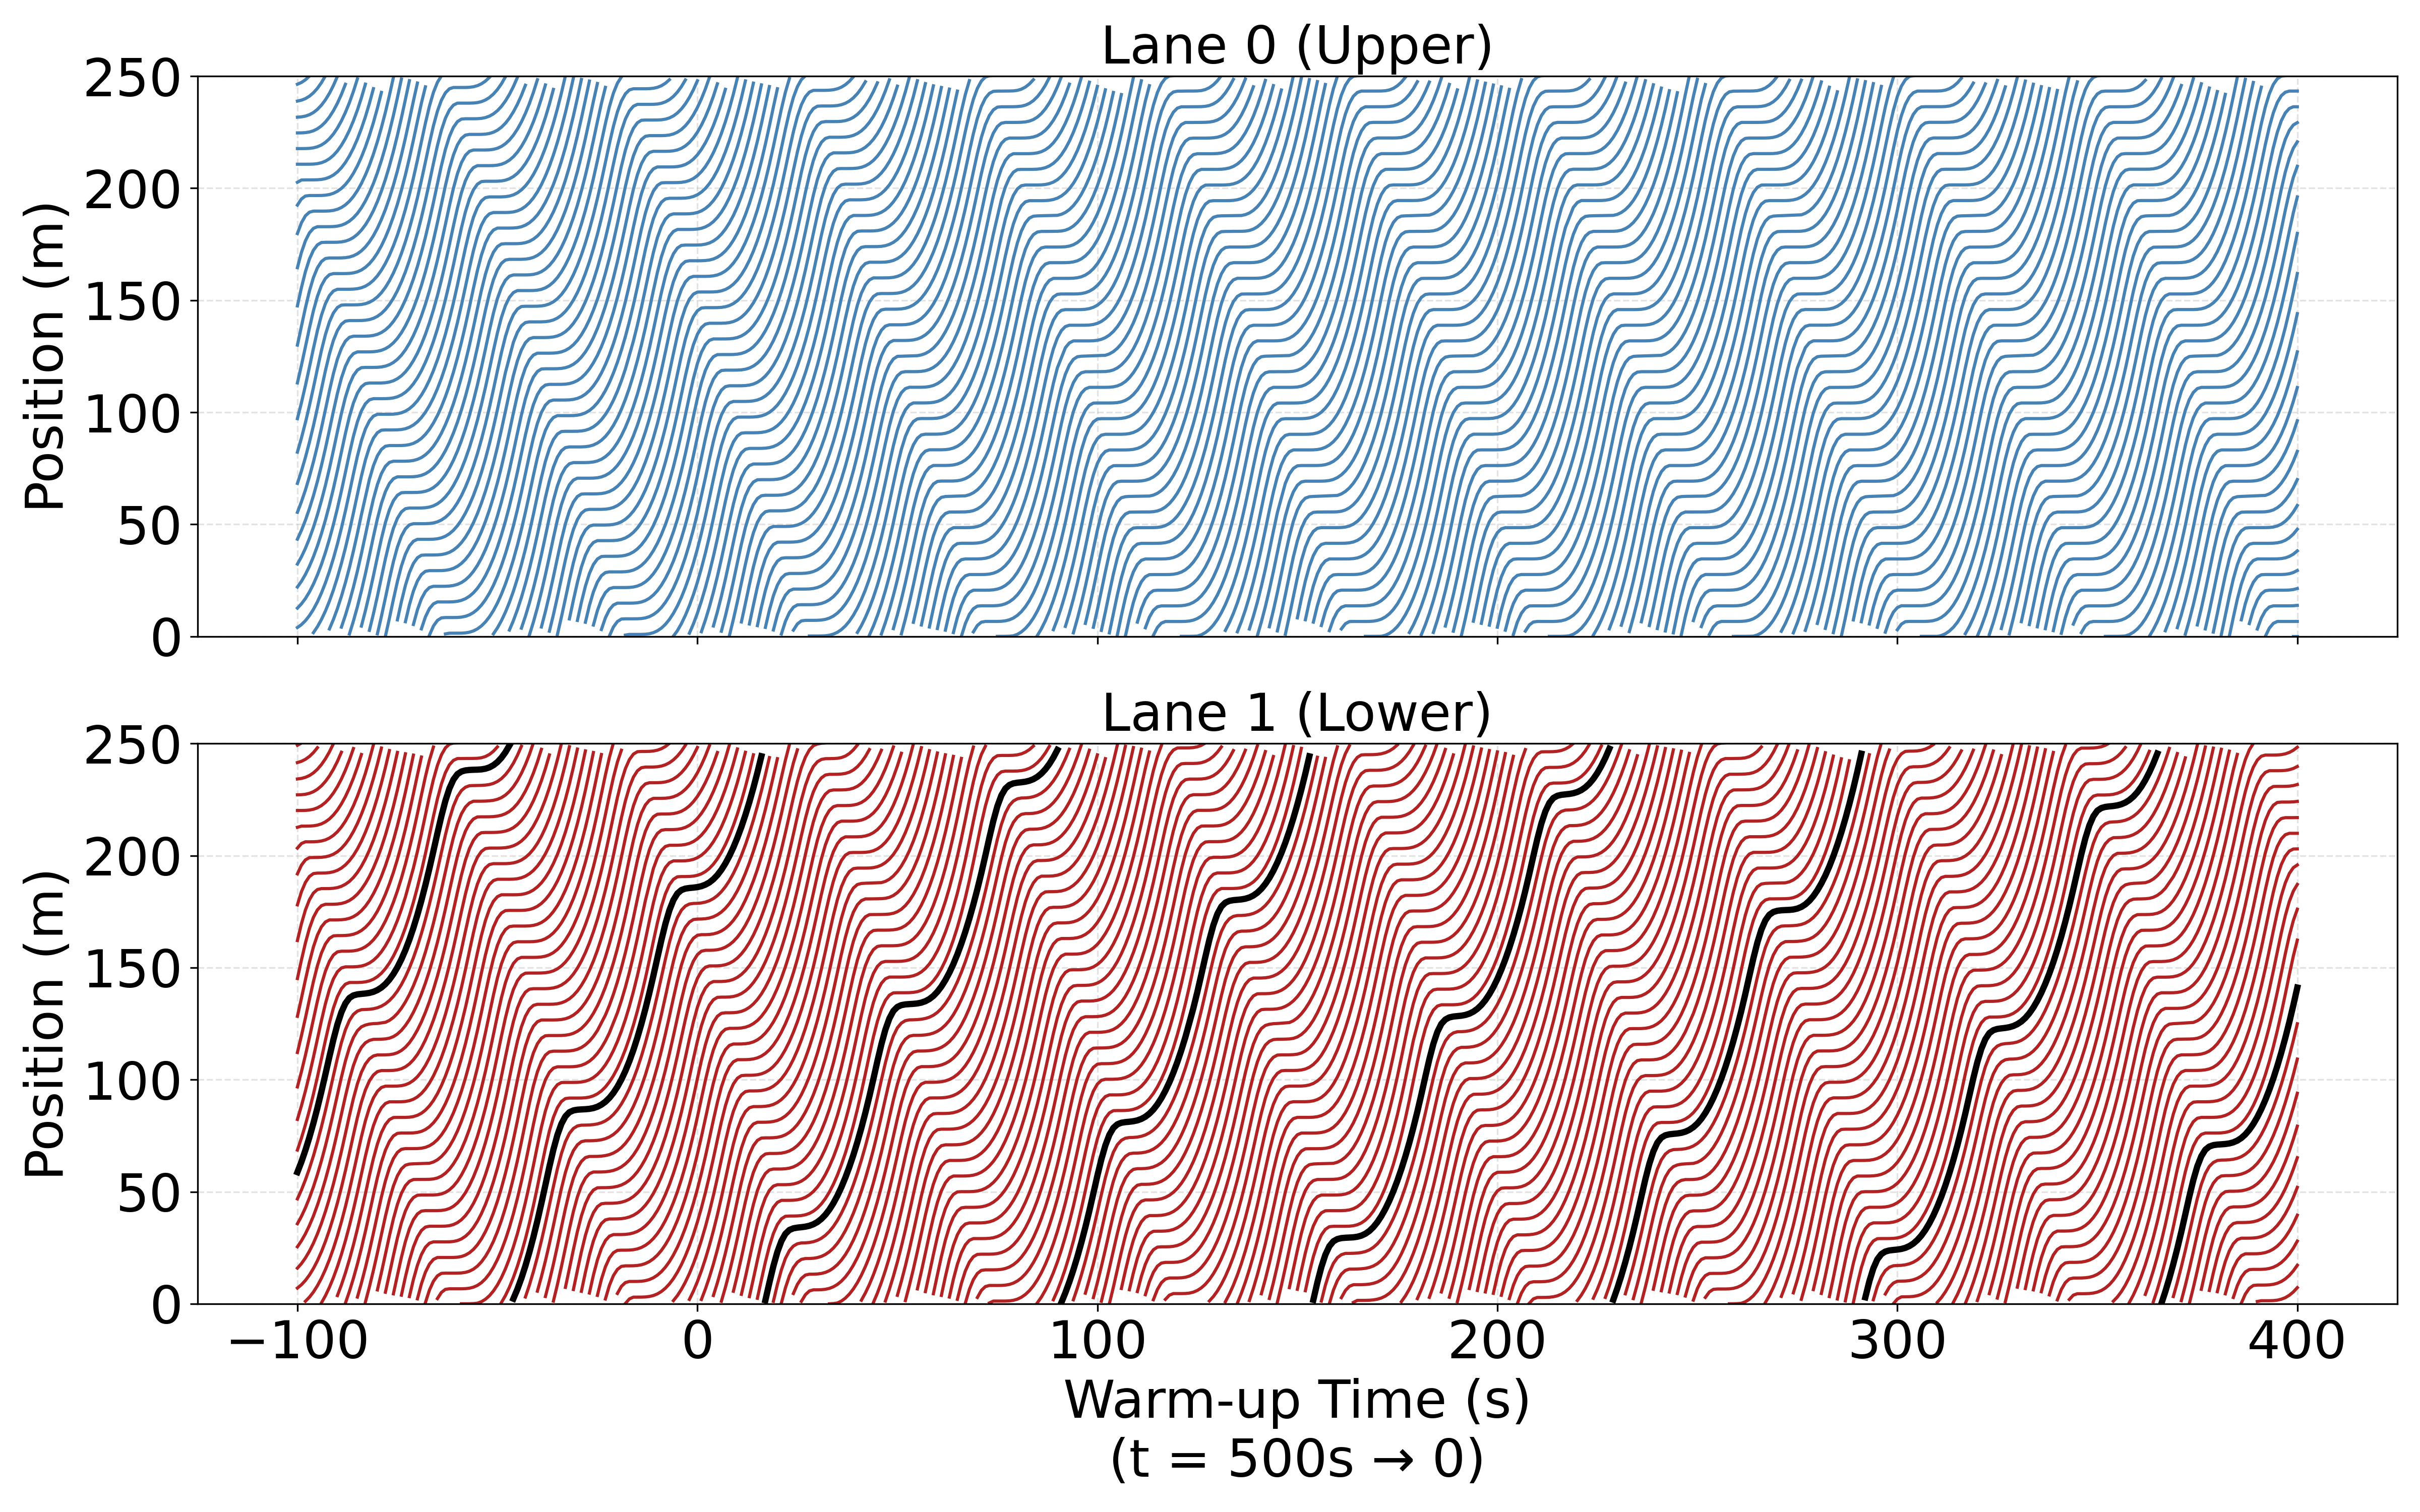
\includegraphics[width=\linewidth,height=3.85cm,keepaspectratio]{../trajectory_log_1AVLC.png}
      \par\smallskip
      \scriptsize\color{UoGTextGray}Compression and expansion persist in both lane trajectories.
    \end{column}
  \end{columns}
  \UoGTakeaway{Richer observation does not compensate for insufficient control authority.}
  \TalkSource{Paper: Single-Agent Results and Analysis; trajectory\_log\_1AVLC.png}
  \note{
    \textbf{Timing:} 0:50

    \textbf{Opening.} The result should not be interpreted simply as failed optimization.

    \textbf{Main explanation.} Close-following is a reasonable response to the reward and the risk of another vehicle merging into the AV gap. The AV reduces some merge opportunities around itself. However, disturbances from the adjacent lane continue to propagate.

    \textbf{Scientific interpretation.} The limitation is structural: one actuator cannot coordinate two moving lane boundaries. This diagnosis motivates a new architecture rather than merely longer training.

    \textbf{Transition.} We therefore introduce a second AV and make cross-lane coordination explicit.

    \textbf{Likely question.} Did the single AV have a lane-change action? Yes, but close-following becomes the dominant learned response and the complete system remains unstable.

    \textbf{Sources.} Docs/ifacconf8pages.tex, Single-Agent Results and Analysis; Docs/trajectory\_log\_1AVLC.png.
  }
\end{frame}

% -----------------------------------------------------------------------------
% Slide 9
% -----------------------------------------------------------------------------
\begin{frame}[shrink=8]{Cooperative RL changes the information and action structure}
  \begin{columns}[T,onlytextwidth]
    \begin{column}{0.64\textwidth}
      \scriptsize
      \begin{align*}
        o_t^i&=\left[
          \frac{v_t^i}{v_{\max}},
          \frac{v_{i,t}^{\mathrm{lead}}}{v_{\max}},
          \frac{v_{i,t}^{\mathrm{foll}}}{v_{\max}},
          \frac{d_{i,t}^{\mathrm{lead}}}{L},
          \frac{d_{i,t}^{\mathrm{foll}}}{L}
        \right],\\[0.18cm]
        o_t&=\left[o_t^1,o_t^2,
          \frac{x_t^1-x_t^2}{L},
          \frac{v_t^1-v_t^2}{v_{\max}}
        \right]\in\mathbb{R}^{12},\\[0.18cm]
        a_t&=\begin{bmatrix}a_1(t)\\a_2(t)\end{bmatrix}\in[-0.5,0.5]^2.
      \end{align*}
    \end{column}
    \begin{column}{0.34\textwidth}
      \begin{itemize}\setlength\itemsep{0.24cm}
        \item Centralized observation
        \item Two longitudinal control inputs
        \item AVs remain in assigned lanes
        \item Pairwise position and velocity are explicit states
      \end{itemize}
      \centering
      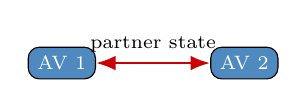
\begin{tikzpicture}[font=\scriptsize]
        \node[draw,rounded corners,fill=UoGBlue!85,text=white] (a) {AV 1};
        \node[draw,rounded corners,fill=UoGBlue!85,text=white,right=1.45cm of a] (b) {AV 2};
        \draw[{Latex}-{Latex},UoGRed,line width=0.9pt] (a)--node[above,text=black]{partner state}(b);
      \end{tikzpicture}
    \end{column}
  \end{columns}
  \UoGTakeaway{The architecture adds direct authority over both lane boundaries.}
  \TalkSource{Paper: Cooperative Reinforcement Learning; singleagent\_ring2AV.py}
  \note{
    \textbf{Timing:} 1:10

    \textbf{Opening.} The cooperative formulation changes both information and action structure.

    \textbf{Main explanation.} Each AV contributes a five-dimensional lane-local observation. Two additional states represent normalized relative position and relative velocity. The full observation is 12-dimensional. Both AVs remain in assigned lanes and control only longitudinal acceleration.

    \textbf{Scientific interpretation.} The controller now has one actuator in each lane and can directly coordinate both moving lane boundaries. The observation is centralized and assumes access to partner state.

    \textbf{Transition.} The reward then determines which form of cooperation is encouraged.

    \textbf{Likely question.} Is the design decentralized? No. Decentralized sensing, communication delay, and packet loss remain future work.

    \textbf{Sources.} Docs/ifacconf8pages.tex, Cooperative Reinforcement Learning; examples/exp\_configs/rl/singleagent/singleagent\_ring2AV.py.
  }
\end{frame}

% -----------------------------------------------------------------------------
% Slide 10
% -----------------------------------------------------------------------------
\begin{frame}[shrink=8]{The cooperative reward explicitly shapes coordination}
  \begin{columns}[T,onlytextwidth]
    \begin{column}{0.62\textwidth}
      \scriptsize
      \begin{align*}
        r_t&=r_{\mathrm{pos},t}+r_{\mathrm{sync},t}+r_{\mathrm{speed},t}+r_{\mathrm{smooth},t},\\
        r_{\mathrm{pos},t}&=-w_{\mathrm{pos}}\left|\frac{x_t^1-x_t^2}{L}\right|,\\
        r_{\mathrm{sync},t}&=-w_{\mathrm{sync}}\left|\frac{v_t^1-v_t^2}{v_{\max}}\right|,\\
        r_{\mathrm{speed},t}&=w_{\mathrm{speed}}\left(\frac{v_t^1+v_t^2}{2v_{\max}}\right)^2,\\
        r_{\mathrm{smooth},t}&=-w_{\mathrm{smooth}}\left[(a_t^1)^2+(a_t^2)^2\right].
      \end{align*}
    \end{column}
    \begin{column}{0.36\textwidth}
      \vspace{0.12cm}
      \small
      \RedLabel{Position} $\rightarrow$ alignment\\[0.22cm]
      \RedLabel{Synchronization} $\rightarrow$ coherent motion\\[0.22cm]
      \RedLabel{Speed} $\rightarrow$ traffic efficiency\\[0.22cm]
      \RedLabel{Smoothness} $\rightarrow$ feasible acceleration
    \end{column}
  \end{columns}
  \vspace{0.18cm}
  \UoGTakeaway{Pairing is reward-shaped learned behavior, not a reward-agnostic emergent phenomenon.}
  \TalkTODO{Retain symbolic weights unless final documented values are supplied.}
  \TalkSource{Paper: Cooperative Reward Design; reviewer comments on reward shaping}
  \note{
    \textbf{Timing:} 1:15

    \textbf{Opening.} The cooperative reward explicitly determines the desired form of coordination.

    \textbf{Main explanation.} The position term favors longitudinal alignment. The synchronization term favors matched velocities. The speed term prevents the pair from optimizing alignment alone, and the smoothness term discourages aggressive acceleration.

    \textbf{Scientific interpretation.} The paired structure is encouraged by the reward and should not be described as reward-agnostic emergence. The current weights are empirically selected. The scientific value lies in using the trained policy to expose a controller structure that can be distilled.

    \textbf{Transition.} The learned behavior suggests a simple geometric mechanism.

    \textbf{Likely question.} Are the reward weights justified by ablation? Not in the current study. Reward ablation and sensitivity analysis are important next experiments.

    \textbf{Sources.} Docs/ifacconf8pages.tex, Cooperative Reward Design; Docs/reviewer\_comments\_summary.md, Reviewer 6 and Reviewer 8 concerns.
  }
\end{frame}

% -----------------------------------------------------------------------------
% Slide 11
% -----------------------------------------------------------------------------
\begin{frame}[shrink=8]{The learned policy suggests a geometric control mechanism}
  \begin{columns}[T,onlytextwidth]
    \begin{column}{0.58\textwidth}
      \centering
      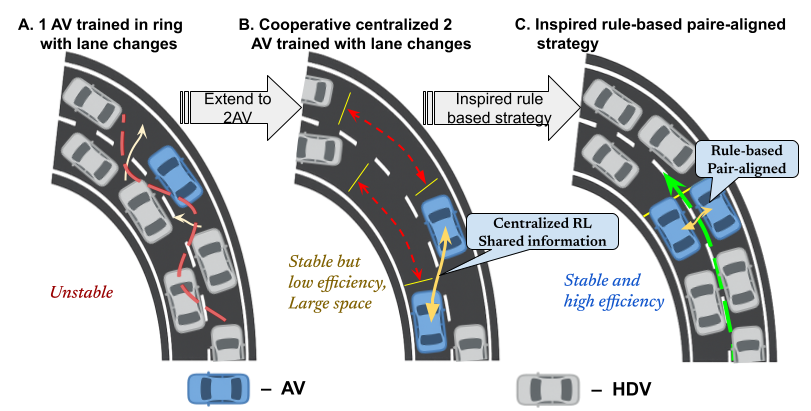
\includegraphics[width=\linewidth,height=4.55cm,keepaspectratio]{../The overview of paired controller for stabilizing flow.png}
    \end{column}
    \begin{column}{0.40\textwidth}
      \textbf{Aligning the AVs removes the staggered gaps used by HDVs to change lanes.}
      \vspace{0.25cm}
      \begin{enumerate}\setlength\itemsep{0.25cm}
        \item The leading AV slows down.
        \item The trailing AV closes the cross-lane offset.
        \item The aligned AVs create a common moving boundary for both lanes.
      \end{enumerate}
    \end{column}
  \end{columns}
  \UoGTakeaway{The two-lane system behaves approximately as one virtual longitudinal lane.}
  \TalkSource{Paper: Cooperative RL Results; overview of paired controller}
  \note{
    \textbf{Timing:} 0:50

    \textbf{Opening.} The trained cooperative policy suggests a geometric control mechanism.

    \textbf{Main explanation.} The leading AV initially reduces speed so the trailing AV can close the longitudinal offset. Once aligned, the two AVs remove the staggered cross-lane gap. HDVs then see a common moving boundary rather than two independent gaps.

    \textbf{Scientific interpretation.} The virtual-lane description refers to coupled longitudinal evolution. It does not mean the physical lanes disappear or that every lane change is undesirable.

    \textbf{Transition.} PARC encodes this geometric mechanism as three explicit control modes.

    \textbf{Likely question.} Could the same mechanism generalize to more lanes? Possibly, but the current evidence covers only two lanes and two AVs.

    \textbf{Sources.} Docs/ifacconf8pages.tex, Cooperative RL Results and Analysis; Docs/The overview of paired controller for stabilizing flow.png.
  }
\end{frame}

% -----------------------------------------------------------------------------
% Slide 12
% -----------------------------------------------------------------------------
\begin{frame}[shrink=8]{PARC encodes the learned mechanism as a hybrid controller}
  \begin{columns}[T,onlytextwidth]
    \begin{column}{0.65\textwidth}
      \small
      \begin{align*}
        d_p&=x_p-x,\qquad \Delta v_p=v_p-v,\\[0.26cm]
        a&=\begin{cases}
          k_{\mathrm{pair}}d_p, & |d_p|>d_{\mathrm{th}},\\[3pt]
          k_{\mathrm{sync}}(v_p-v), & |v_p-v|>\delta_v,\\[3pt]
          k_v(v^\star-v), & \text{otherwise},
        \end{cases}\\[0.26cm]
        a&\leftarrow\operatorname{clip}(a,-a_{\max},a_{\max}).
      \end{align*}
    \end{column}
    \begin{column}{0.33\textwidth}
      \vspace{0.18cm}
      \RedLabel{Formation}\\
      Regulate cross-lane position error.\\[0.38cm]
      \RedLabel{Synchronization}\\
      Remove relative velocity.\\[0.38cm]
      \RedLabel{Cruise}\\
      Track the shared equilibrium speed.
    \end{column}
  \end{columns}
  \UoGTakeaway{The controller separates geometry, coherent motion, and efficient cruise.}
  \TalkSource{Paper: PARC strategy and Algorithm 1}
  \note{
    \textbf{Timing:} 1:20

    \textbf{Opening.} PARC converts the learned behavior into three explicit control modes.

    \textbf{Main explanation.} Define d-p as the signed periodic longitudinal displacement to the designated partner. During formation, proportional feedback reduces cross-lane position error. During synchronization, relative velocity is removed after positional alignment. During cruise, both AVs track a common equilibrium speed. All commands are clipped to physical acceleration limits.

    \textbf{Scientific interpretation.} The hierarchy makes the mechanism inspectable and separates three tasks that the learned policy blends together. The paper reports simulation evidence rather than a formal hybrid-system stability proof.

    \textbf{Transition.} The final control mode requires a traffic-consistent target speed.

    \textbf{Likely question.} How are gains and thresholds selected? They are design parameters in the present study; a systematic sensitivity analysis is future work.

    \textbf{Sources.} Docs/ifacconf8pages.tex, Rule-Based Pair-Aligned Control Strategy and Algorithm 1.
  }
\end{frame}

% -----------------------------------------------------------------------------
% Slide 13
% -----------------------------------------------------------------------------
\begin{frame}[shrink=8]{The cruising speed follows the equilibrium traffic geometry}
  \begin{columns}[T,onlytextwidth]
    \begin{column}{0.62\textwidth}
      \small
      \begin{align*}
        \textcolor{UoGRed}{N_\ell}&=\frac{N_{\mathrm{total}}}{2}=22,\\[0.18cm]
        s_{\mathrm{eq}}^{\max}&=\frac{L-N_\ell s_{\min}}{N_\ell-1},\\[0.28cm]
        s_{\mathrm{eq}}^{\max}
        &=\left(s_0+\textcolor{UoGRed}{v^\star}\tau\right)
        \left[1-\left(\frac{\textcolor{UoGRed}{v^\star}}{v_0}\right)^\gamma\right]^{-1/2}.
      \end{align*}
    \end{column}
    \begin{column}{0.36\textwidth}
      \begin{itemize}\setlength\itemsep{0.30cm}
        \item Road geometry determines feasible equilibrium spacing.
        \item The IDM relation maps spacing to the shared target speed $v^\star$.
        \item Both AVs track the same $v^\star$ after pairing.
      \end{itemize}
    \end{column}
  \end{columns}
  \UoGTakeaway{The cruise target respects the density of the effective lane, not only the road speed limit.}
  \TalkSource{Paper: cruise-speed derivation; paired\_ring.py v\_eq\_max\_function}
  \note{
    \textbf{Timing:} 0:50

    \textbf{Opening.} The target speed is not simply set to the road speed limit.

    \textbf{Main explanation.} Dense traffic restricts the speed compatible with uniform equilibrium spacing. The implementation computes the equilibrium speed using the effective number of vehicles per lane. With 44 total vehicles and two lanes, it uses N-l equal to 22. The nonlinear IDM relation is then solved numerically for v-star.

    \textbf{Scientific interpretation.} This links network geometry and car-following equilibrium directly to the rule-based cruise mode.

    \textbf{Transition.} We now compare methods chosen to isolate the value of each methodological step.

    \textbf{Likely question.} Why use a per-lane count? The implementation evaluates the equilibrium of the virtual longitudinal lane using TOTAL\_VEH divided by LANES.

    \textbf{Sources.} Docs/ifacconf8pages.tex, PARC cruise-speed derivation; examples/exp\_configs/non\_rl/paired\_ring.py, num\_per\_lane and v\_eq\_max\_function.
  }
\end{frame}

% -----------------------------------------------------------------------------
% Slide 14
% -----------------------------------------------------------------------------
\begin{frame}{The validation isolates the value of each methodological step}
  \begin{columns}[T,onlytextwidth]
    \begin{column}{0.58\textwidth}
      \scriptsize
      \renewcommand{\arraystretch}{1.40}
      \begin{tabularx}{\linewidth}{>{\bfseries\raggedright\arraybackslash}p{0.25\linewidth} >{\raggedright\arraybackslash}X}
        \toprule
        \textcolor{UoGRed}{Method} & \textcolor{UoGRed}{Scientific purpose}\\
        \midrule
        All-HDV & Demonstrate uncontrolled waves\\
        RL-1AV & Test whether one learned AV is sufficient\\
        RL-Coop-2AV & Test whether shared information creates useful coordination\\
        2AV-SLC & Control for AV count without cross-lane coordination\\
        PARC & Test the distilled pair-aligned mechanism\\
        \bottomrule
      \end{tabularx}
    \end{column}
    \begin{column}{0.40\textwidth}
      \centering
      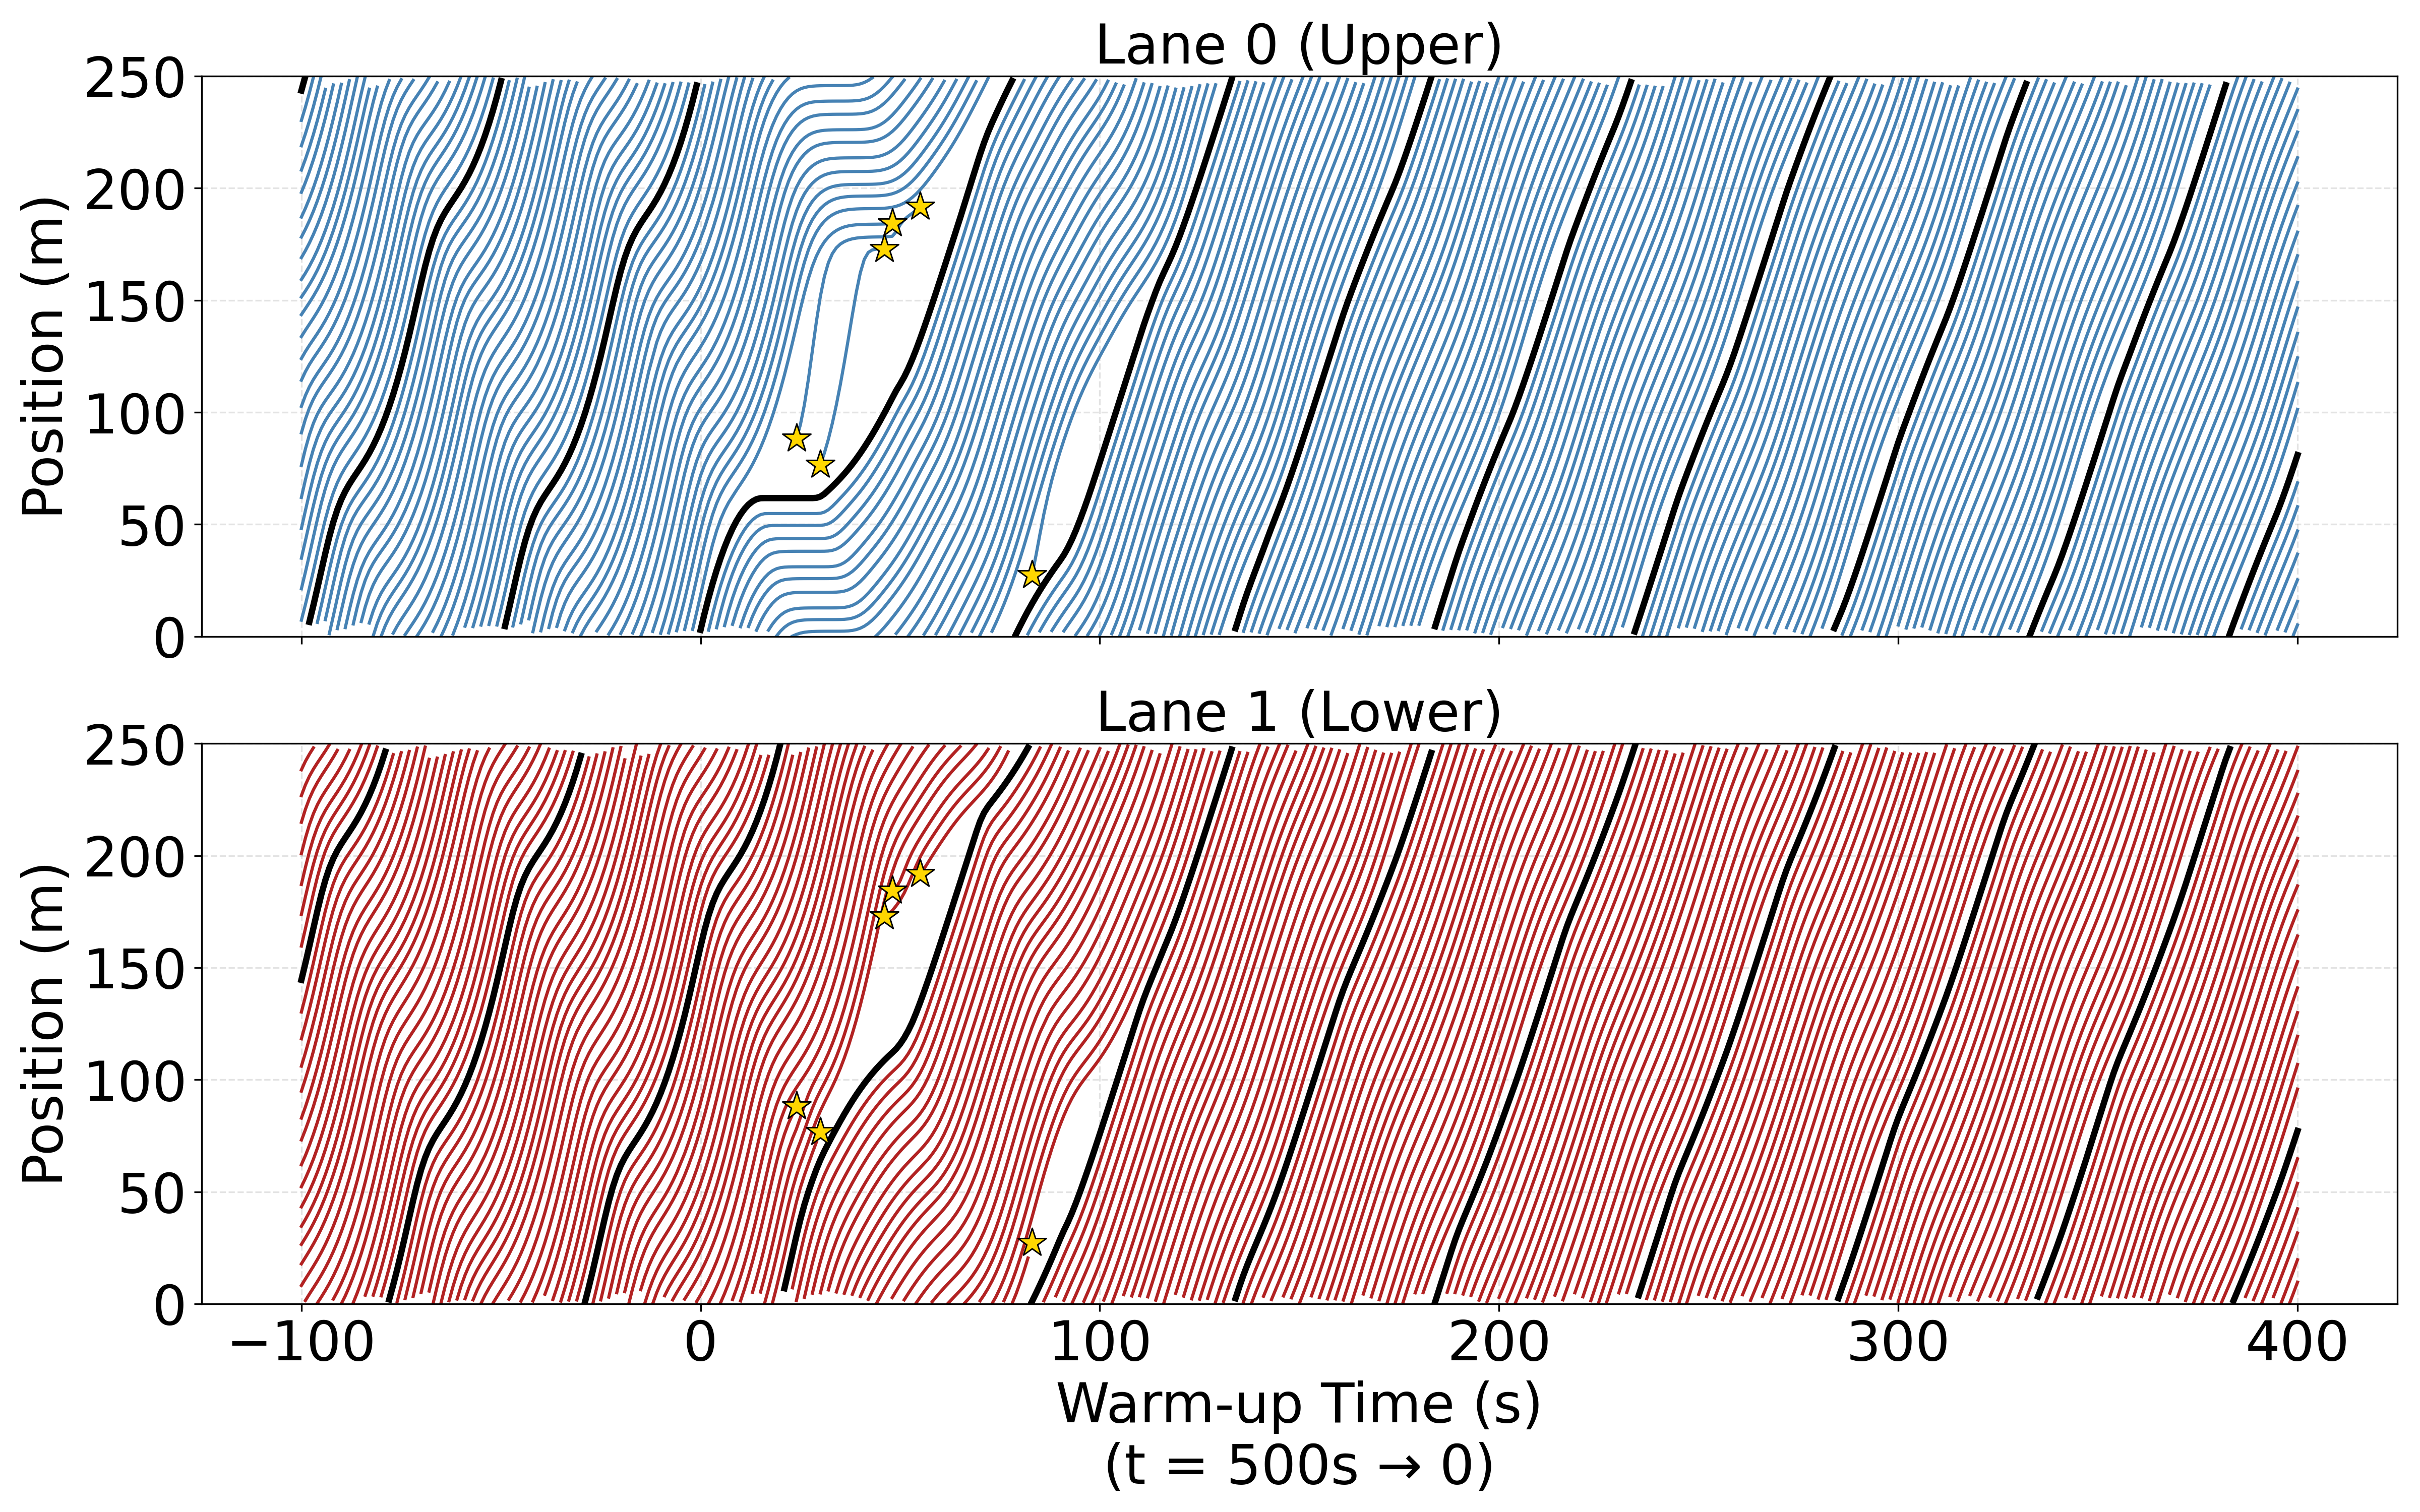
\includegraphics[width=\linewidth,height=4.45cm,keepaspectratio]{../trajectory_log_paired_controller.png}
      \scriptsize\color{UoGRed}\bfseries After alignment: nearly parallel trajectories
    \end{column}
  \end{columns}
  \TalkSource{Paper: Discussion and Comparison; trajectory\_log\_paired\_controller.png}
  \note{
    \textbf{Timing:} 0:55

    \textbf{Opening.} Each baseline answers a separate methodological question.

    \textbf{Main explanation.} All-HDV demonstrates the uncontrolled phenomenon. RL-1AV tests the classical single-actuator extension. RL-Coop-2AV tests whether shared information enables coordination. 2AV-SLC is the most important fair baseline because it uses the same number of AVs as PARC without partner coordination. PARC tests whether the distilled mechanism is sufficient.

    \textbf{Scientific interpretation.} Nearly parallel time-space trajectories indicate steady motion. The comparison separates the effect of adding AVs from the effect of coordinating them.

    \textbf{Transition.} The comparison shows that coordination, rather than AV count alone, produces the improvement.

    \textbf{Likely question.} Why is 1AV-SLC not the primary baseline? It does not stabilize the adjacent lane, so it does not solve the complete two-lane problem.

    \textbf{Sources.} Docs/ifacconf8pages.tex, Discussion and Comparison; Docs/trajectory\_log\_paired\_controller.png.
  }
\end{frame}

% -----------------------------------------------------------------------------
% Slide 15
% -----------------------------------------------------------------------------
\begin{frame}[shrink=8]{RL identifies the structure; PARC executes it efficiently}
  \begin{columns}[T,onlytextwidth]
    \begin{column}{0.49\textwidth}
      \centering
      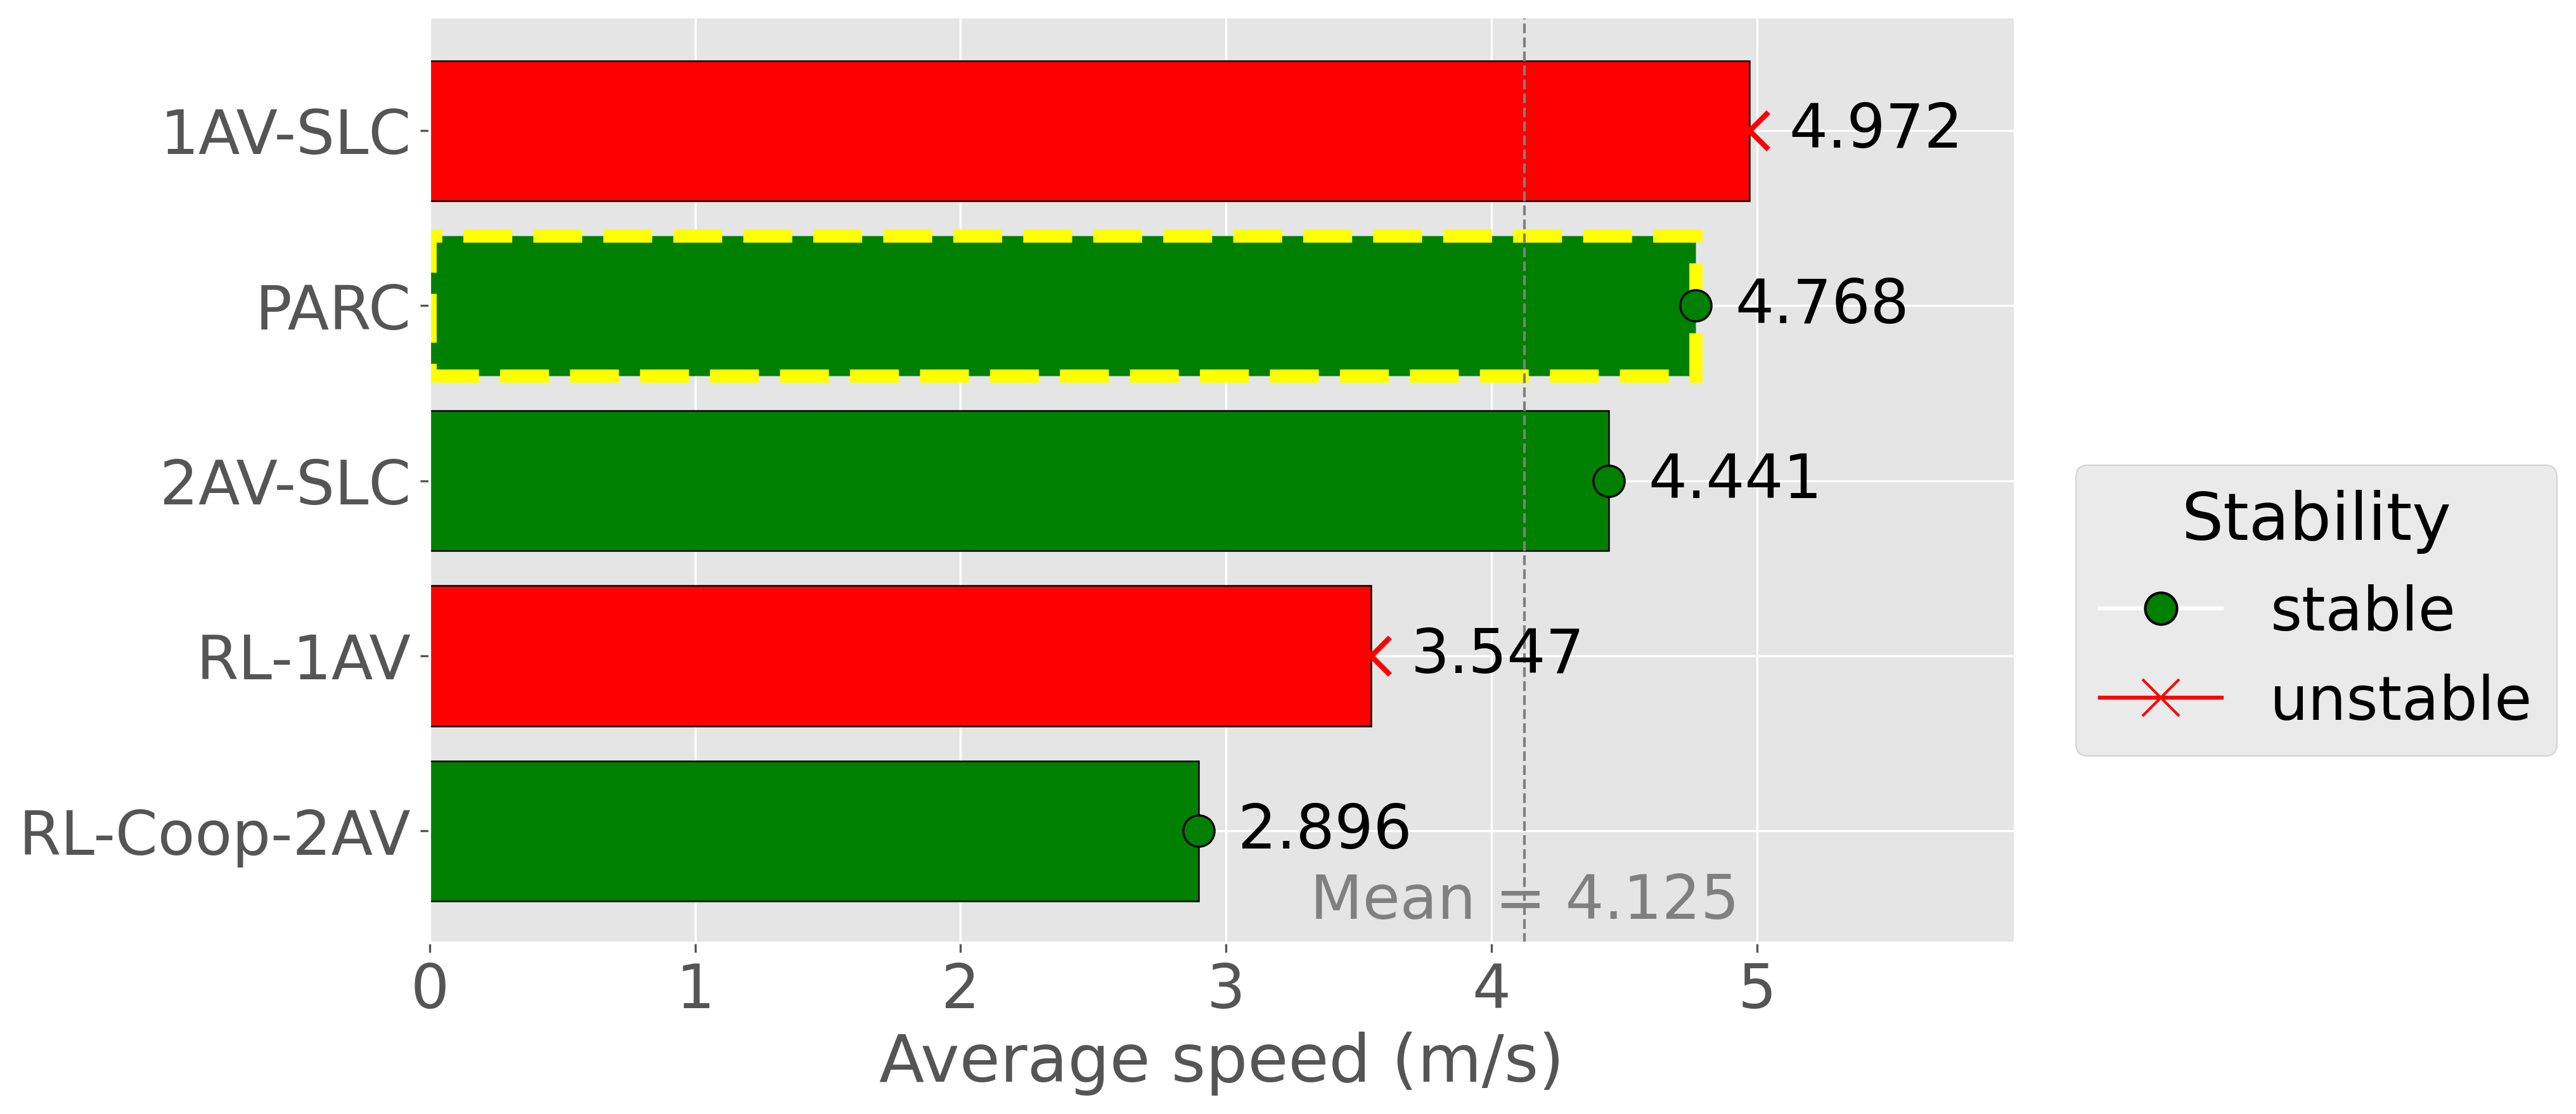
\includegraphics[width=\linewidth,height=4.15cm,keepaspectratio]{../avg_speed_comparison.png}
    \end{column}
    \begin{column}{0.49\textwidth}
      \centering
      \large
      $4.441\,\mathrm{m/s}\quad\longrightarrow\quad4.768\,\mathrm{m/s}$

      \vspace{0.12cm}
      \normalsize
      $\displaystyle\frac{4.768-4.441}{4.441}\times100\%=\textcolor{UoGRed}{\mathbf{7.4\%}}$

      \vspace{0.22cm}
      \small\raggedright
      \begin{enumerate}\setlength\itemsep{0.14cm}
        \item One AV cannot reject lane-changing disturbances across both lanes.
        \item Cooperative reward design identifies cross-lane alignment as a useful structure.
        \item PARC implements that structure transparently and improves stabilized speed.
      \end{enumerate}
    \end{column}
  \end{columns}
  \scriptsize\color{UoGTextGray}Current evidence is limited to centralized information, two lanes, two AVs, and simulation-based validation.
  \TalkSource{Paper: Discussion and Conclusion; avg\_speed\_comparison.png; reviewer comments}
  \note{
    \textbf{Timing:} 0:45

    \textbf{Opening.} The fair quantitative comparison is PARC versus 2AV-SLC.

    \textbf{Main explanation.} Both methods use two AVs and address both lanes. PARC increases stabilized average speed from 4.441 to 4.768 metres per second, corresponding to approximately 7.4 percent. 1AV-SLC reports 4.972 metres per second, but it does not stabilize the adjacent lane. Cooperative RL stabilizes both lanes but operates conservatively because of reward weighting.

    \textbf{Scientific interpretation.} RL serves as a design instrument, and PARC becomes the interpretable runtime controller. The current evidence is limited to centralized information, two lanes, two AVs, no optimality proof, and no explicit energy, safety, or comfort evaluation.

    \textbf{Transition.} Before questions, I would like to highlight the next IFAC World Congress.

    \textbf{Likely question.} Is PARC optimal? No. The result demonstrates relative improvement over selected baselines, not system optimality.

    \textbf{Sources.} Docs/ifacconf8pages.tex, Discussion, Comparison, and Conclusion; Docs/avg\_speed\_comparison.png; Docs/reviewer\_comments\_summary.md.
  }
\end{frame}

% -----------------------------------------------------------------------------
% Slide 16
% -----------------------------------------------------------------------------
\begin{frame}[plain,noframenumbering]
  \begin{tikzpicture}[remember picture,overlay]
    \node[anchor=center,inner sep=0] at (current page.center)
      {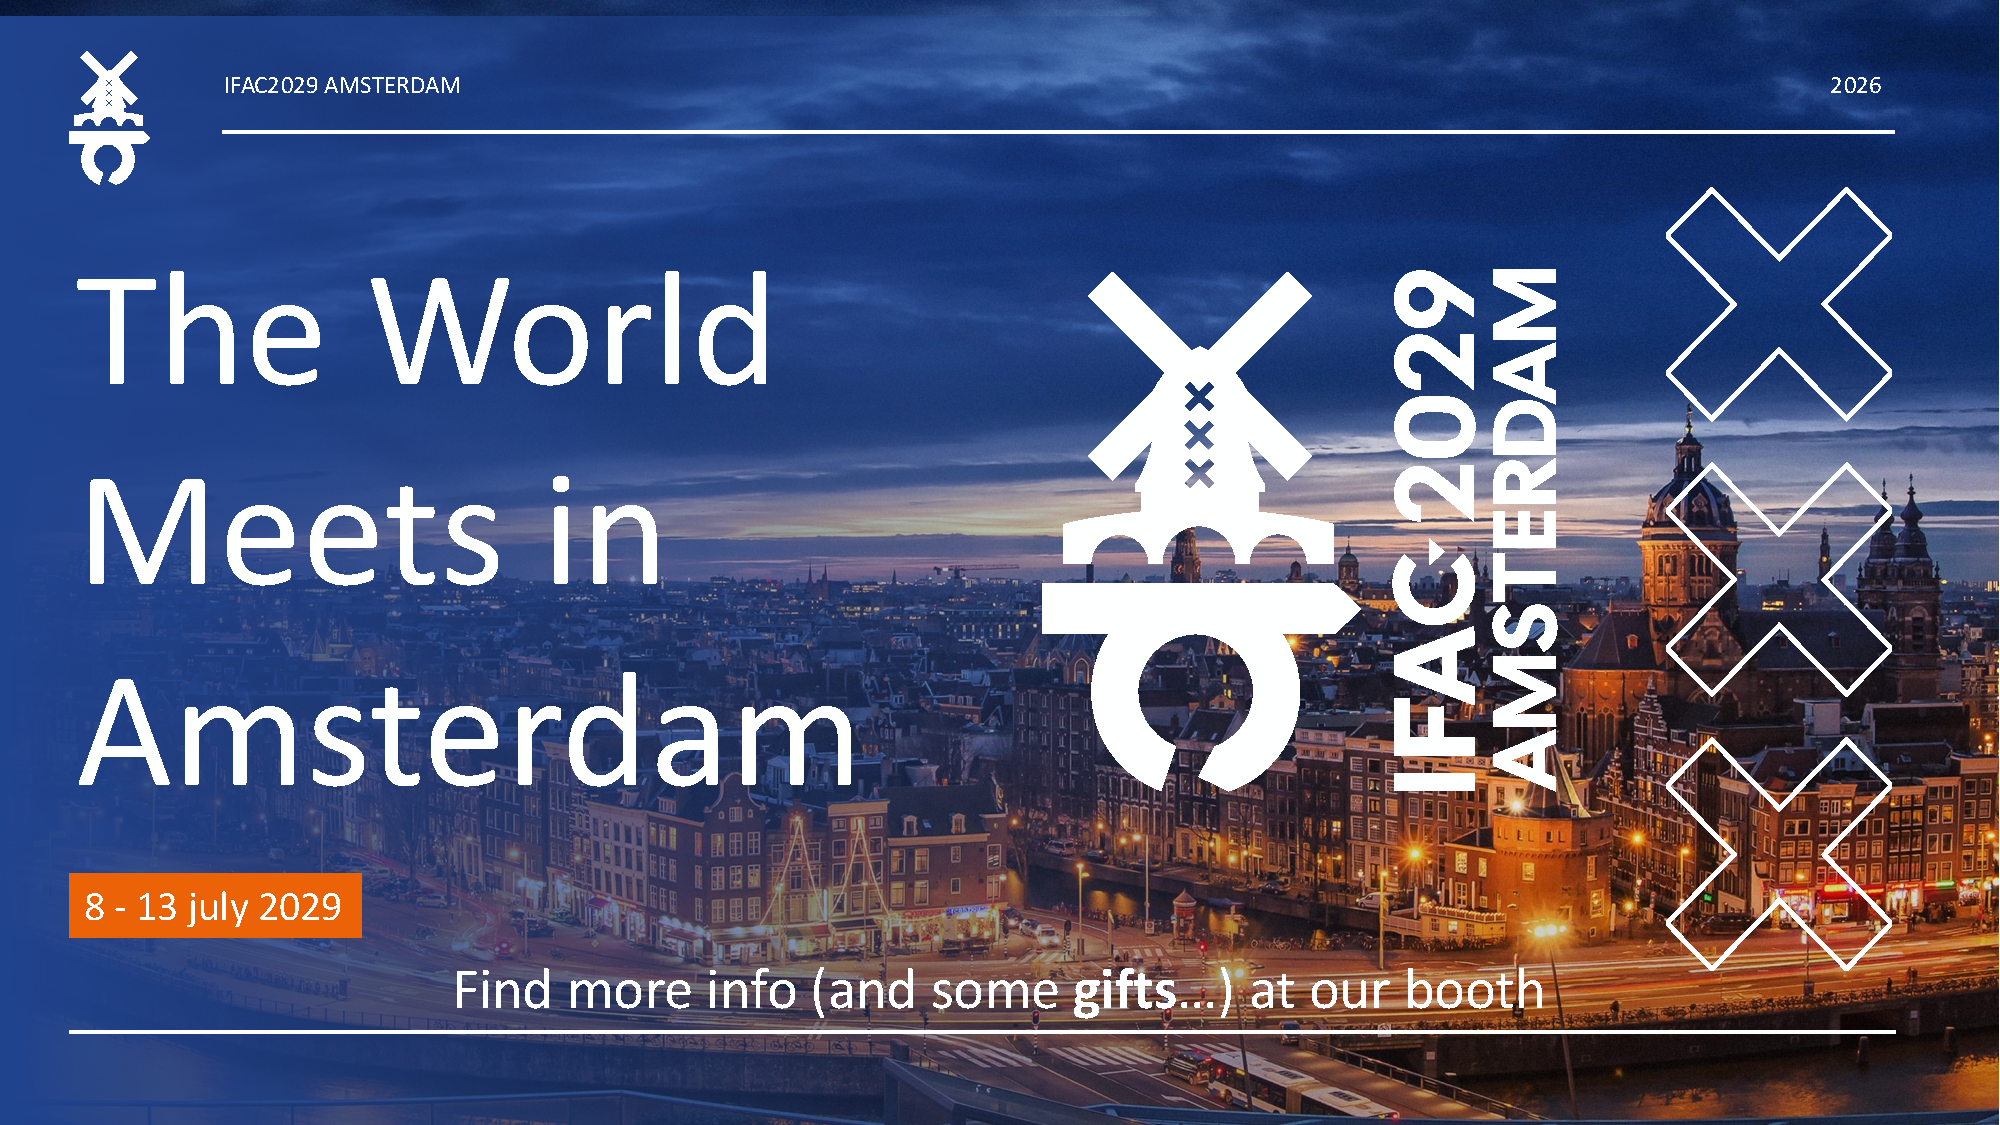
\includegraphics[width=\paperwidth,height=\paperheight]{../../IFAC29.Advertising.pdf}};
  \end{tikzpicture}
  \note{
    \textbf{Timing:} 0:20

    \textbf{Opening.} The next IFAC World Congress will take place in Amsterdam from 8 to 13 July 2029.

    \textbf{Main explanation.} We look forward to welcoming the IFAC community to the Netherlands. Please visit the IFAC 2029 booth for further information.

    \textbf{Scientific interpretation.} This is the official supplied IFAC 2029 advertisement and is intentionally shown unchanged.

    \textbf{Transition.} Thank you. I welcome your questions.

    \textbf{Likely question.} Where can I find more information? At the IFAC 2029 booth and through future official congress announcements.

    \textbf{Sources.} IFAC29.Advertising.pdf.
  }
\end{frame}

\end{document}
